% !TeX program = xelatex
\documentclass[aspectratio=43]{beamer}
\usepackage{../plantilla-diapositivas/tema-maestria}
\usepackage{graphicx}
\usepackage{booktabs}
\usepackage[spanish,es-noshorthands]{babel}
\usepackage{tikz}

% ---------------- Navegacion y pie de esta presentacion ----------------
\setnav{5}{{Introducción},{Datos},{Modelos},{Resultados},{Conclusiones}}
\setfootizq{Maestría en Ciencia de Datos}
\setfootder{Algoritmos de Clasificación en R}

\title{Práctica 7 -- Algoritmos de Clasificación en R}
\author{Miguel Angel Deza Cuela}
\date{Septiembre, 2026}

% Caja de codigo R (sin verbatim, para no necesitar frames [fragile])
\newcommand{\codigoR}[1]{%
  \begin{center}
  \tikz\node[fill=white, draw=cNavy, line width=0.6pt, rounded corners=4pt,
             inner xsep=8pt, inner ysep=5pt, text width=0.88\linewidth, align=left,
             font=\ttfamily\scriptsize] {#1};
  \end{center}%
}

% Circulo con icono (para la fila de algoritmos)
\newcommand{\circuloicono}[3]{%
  % #1 = icono kebab, #2 = titulo, #3 = subtitulo
  \begin{minipage}[t]{0.19\textwidth}
    \centering
    \tikz\node[circle, fill=cNavy, minimum size=1.05cm, inner sep=0pt]
      {\textcolor{white}{\large\faIcon{#1}}};\\[3pt]
    {\small\bfseries\color{cNavy} #2}\\
    {\scriptsize #3}
  \end{minipage}%
}

\begin{document}

% ============================================================
% 1. PORTADA
% ============================================================
\activarnav{1}
\begin{frame}
  \vspace{0.15cm}
  \portadapill{Práctica 7\\ Algoritmos de Clasificación en R}

  \vspace{0.3cm}
  \begin{center}
    {\bfseries\large Presentado por:}\\[2pt]
    {\large Miguel Angel Deza Cuela}
  \end{center}

  \vspace{0.25cm}
  \begin{center}
  \begin{tabular}{@{}l l@{}}
    \textcolor{cNavy}{\faIcon{graduation-cap}} & Maestría en Ciencia de Datos -- UNSA \\[4pt]
    \textcolor{cNavy}{\faIcon{book}} & Introducción a Ciencia de Datos \\[4pt]
    \textcolor{cNavy}{\faIcon{chalkboard-teacher}} & Docente: Yessenia Deysi Yari Ramos \\[4pt]
    \textcolor{cNavy}{\faIcon{map-marker-alt}} & Arequipa, Perú \\[4pt]
    \textcolor{cNavy}{\faIcon{calendar-alt}} & Septiembre, 2026 \\
  \end{tabular}
  \end{center}
\end{frame}

% ============================================================
% 2. OBJETIVO Y DATASET
% ============================================================
\activarnav{1}
\begin{frame}
  \seccionpill{\faIcon{bullseye}\ \ Objetivo y dataset elegido}
  \vspace{0.2cm}

  \begin{columns}[T]
    \begin{column}{0.55\textwidth}
      \itemcheck{Objetivo}{Explorar y comparar cinco algoritmos de clasificación en R
        con el paquete \textbf{caret}.}
      \itemcheck{Obesity Levels (Kaggle)}{Nivel de obesidad de personas de
        \textbf{México, Perú y Colombia} según sus hábitos alimenticios y actividad física.}
      \itemcheck{Tamaño}{\textbf{2111 personas}, 16 predictores y la clase
        \texttt{NObeyesdad} con \textbf{7 niveles}.}
      \itemcheck{Calidad}{Sin valores faltantes y con clases balanceadas
        (12.9\,\% -- 16.6\,\% por nivel).}
    \end{column}
    \begin{column}{0.43\textwidth}
      \centering
      \vspace{0.3cm}
      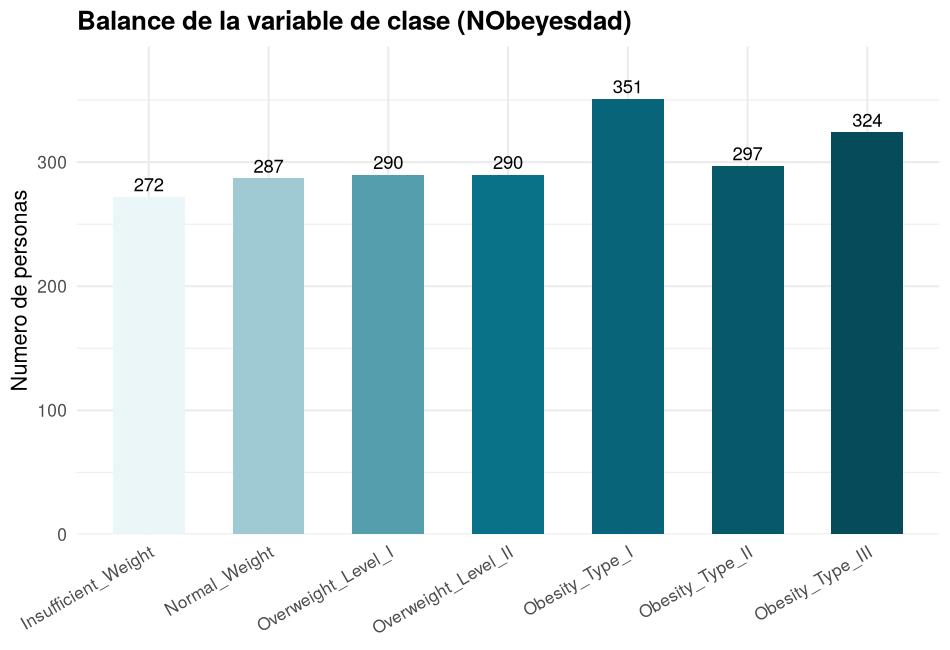
\includegraphics[width=\linewidth]{img/grafico-balance-clases.png}\\
      {\scriptsize\color{cNavy} Balance de la variable de clase}
    \end{column}
  \end{columns}
\end{frame}

% ============================================================
% 3. ANALISIS EXPLORATORIO
% ============================================================
\activarnav{2}
\begin{frame}
  \seccionpill{\faIcon{search}\ \ Análisis exploratorio}
  \vspace{0.15cm}

  \begin{center}
    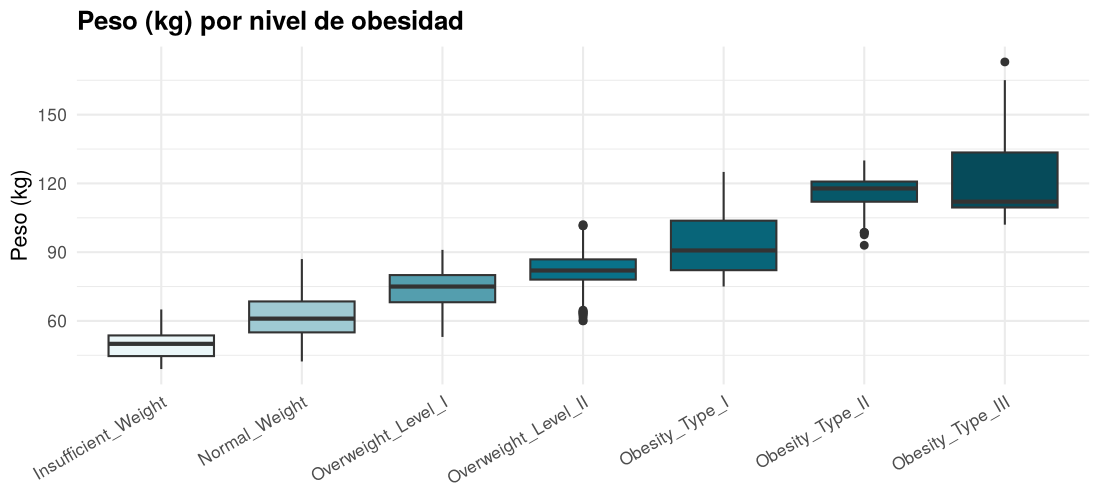
\includegraphics[width=0.9\linewidth]{img/grafico-boxplots-variables.png}
  \end{center}

  \vspace{-4pt}
  \begin{columns}[T]
    \begin{column}{0.5\textwidth}
      \itemcheck{Peso vs. nivel}{La relación es monótona: a más peso, mayor nivel de
        obesidad (la clase se construye a partir del IMC).}
    \end{column}
    \begin{column}{0.5\textwidth}
      \itemcheck{Correlaciones}{\texttt{Height}--\texttt{Weight} es la más fuerte (0.46);
        \texttt{Age}--\texttt{TUE} la única negativa relevante (-0.30).}
    \end{column}
  \end{columns}
\end{frame}

% ============================================================
% 4. CORRELACION + PREPROCESAMIENTO
% ============================================================
\activarnav{2}
\begin{frame}
  \seccionpill{\faIcon{tools}\ \ Preprocesamiento}
  \vspace{0.15cm}

  \begin{columns}[T]
    \begin{column}{0.44\textwidth}
      \centering
      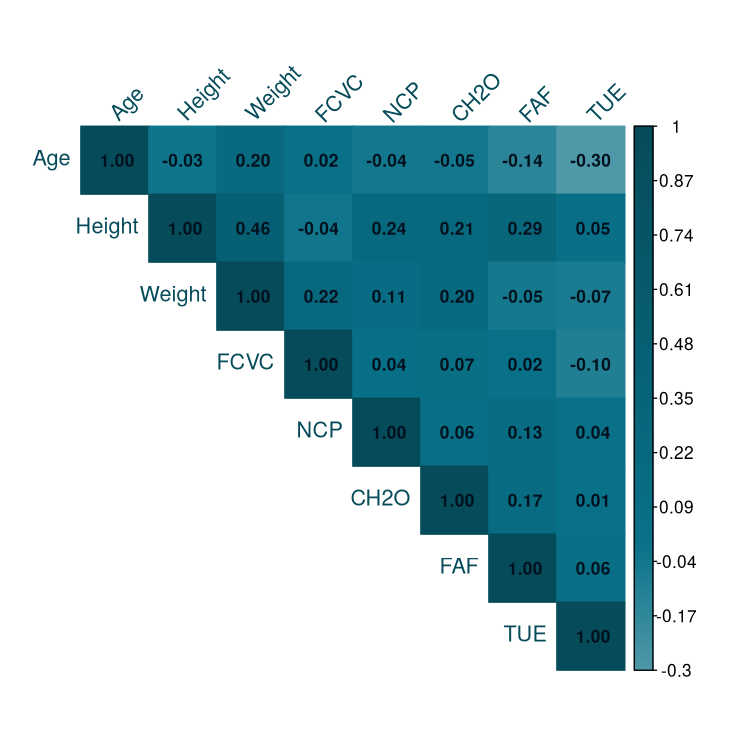
\includegraphics[width=\linewidth]{img/grafico-correlacion.png}\\
      {\scriptsize\color{cNavy} Correlación entre predictores numéricos}
    \end{column}
    \begin{column}{0.54\textwidth}
      \itemcheck{Sin imputación}{No hay valores \texttt{NA} en ninguna de las 17 columnas.}
      \itemcheck{Categóricas a dummies}{Las 8 columnas categóricas quedan como
        \texttt{factor} y \texttt{train()} las convierte a variables dummy.}
      \itemcheck{Centrado y escalado}{Necesario para kNN y SVM, que son sensibles a la
        escala de las variables.}
      \itemcheck{Partición 80/20}{1691 filas de entrenamiento y 420 de prueba, estratificadas
        con \texttt{createDataPartition}.}
    \end{column}
  \end{columns}
\end{frame}

% ============================================================
% 5. ALGORITMOS
% ============================================================
\activarnav{3}
\begin{frame}
  \seccionpill{\faIcon{cogs}\ \ Algoritmos ejecutados}
  \vspace{0.3cm}

  \begin{center}
    \circuloicono{project-diagram}{LDA}{Discriminante lineal}\hfill
    \circuloicono{sitemap}{CART}{Árbol de decisión}\hfill
    \circuloicono{users}{kNN}{k vecinos}\hfill
    \circuloicono{grip-lines}{SVM}{Kernel lineal}\hfill
    \circuloicono{tree}{RF}{Random Forest}
  \end{center}

  \vspace{0.2cm}
  {\footnotesize Todos con la misma validación cruzada: \textbf{10 pliegues $\times$ 3
  repeticiones}, métrica \textbf{Accuracy}:}

  \codigoR{%
  control \textless- trainControl(method = "repeatedcv",\\
  \hspace*{24ex}number = 10, repeats = 3)\\[2pt]
  fit \textless- train(NObeyesdad \textasciitilde{} ., data = train, method = m,\\
  \hspace*{9ex}metric = "Accuracy", trControl = control)\\[2pt]
  {\color{cLimeDark}\# m = "lda", "rpart", "knn", "svmLinear", "rf"}}
\end{frame}

% ============================================================
% 6. RESULTADOS: TABLA + CV
% ============================================================
\activarnav{4}
\begin{frame}
  \seccionpill{\faIcon{chart-bar}\ \ Evaluación de los algoritmos}
  \vspace{0.1cm}

  \begin{center}
  \footnotesize
  \begin{tabular}{lrrrrr}
    \toprule
    \textbf{Modelo} & \textbf{Acc. CV} & \textbf{Acc. test} & \textbf{Kappa} & \textbf{Sensib.} & \textbf{Especif.} \\
    \midrule
    LDA           & 0.896 & 0.879 & 0.858 & 0.875 & 0.980 \\
    CART          & 0.777 & 0.783 & 0.747 & 0.789 & 0.964 \\
    kNN           & 0.790 & 0.819 & 0.789 & 0.815 & 0.970 \\
    SVM lineal    & 0.951 & 0.943 & 0.933 & 0.941 & 0.991 \\
    \textcolor{cNavy}{\textbf{Random Forest}} & \textbf{0.965} & \textbf{0.969} & \textbf{0.964} & \textbf{0.969} & \textbf{0.995} \\
    \bottomrule
  \end{tabular}
  \end{center}

  \begin{columns}[T]
    \begin{column}{0.52\textwidth}
      \centering
      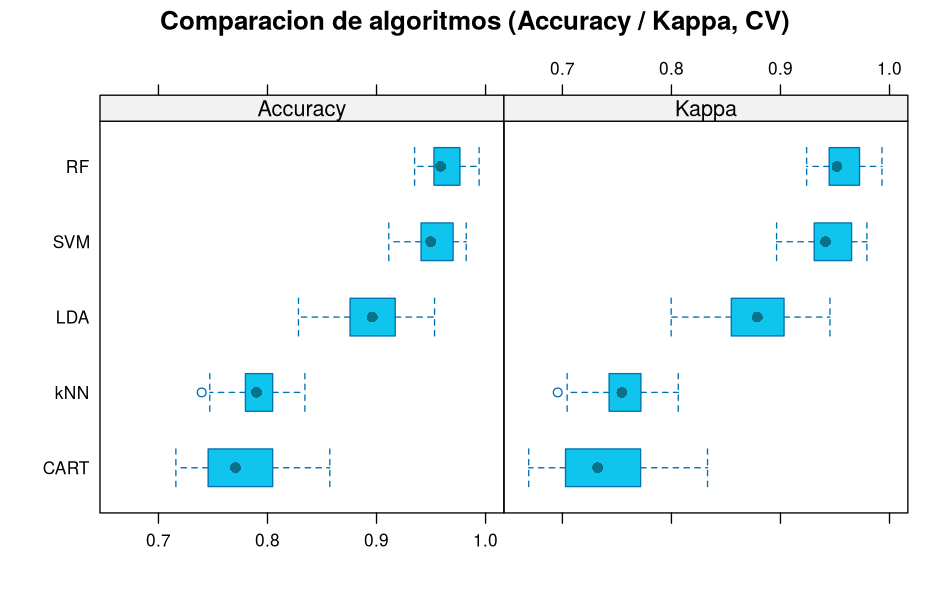
\includegraphics[width=\linewidth]{img/grafico-comparacion-cv.png}
    \end{column}
    \begin{column}{0.46\textwidth}
      \itemcheck{Ganador: Random Forest}{96.9\,\% de accuracy en prueba (420 personas).}
      \itemcheck{Jerarquía clara}{RF $>$ SVM $>$ LDA $>$ kNN $>$ CART, igual en CV y en
        el conjunto de prueba.}
    \end{column}
  \end{columns}
\end{frame}

% ============================================================
% 7. INTERPRETACION
% ============================================================
\activarnav{4}
\begin{frame}
  \seccionpill{\faIcon{tree}\ \ ¿Qué aprendieron los modelos?}
  \vspace{0.15cm}

  \begin{columns}[T]
    \begin{column}{0.5\textwidth}
      \centering
      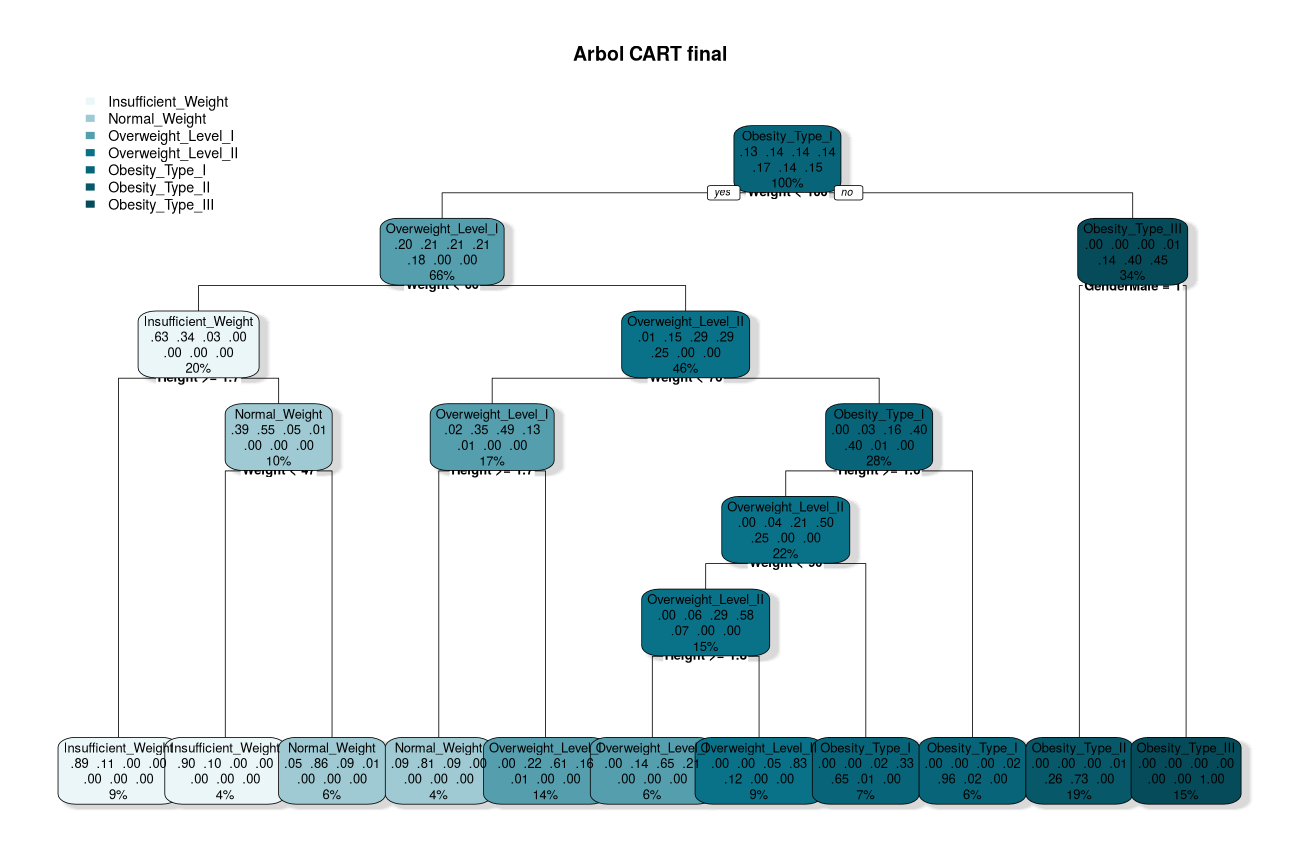
\includegraphics[width=\linewidth]{img/grafico-arbol-cart.png}\\
      {\scriptsize\color{cNavy} Árbol CART final}
    \end{column}
    \begin{column}{0.48\textwidth}
      \centering
      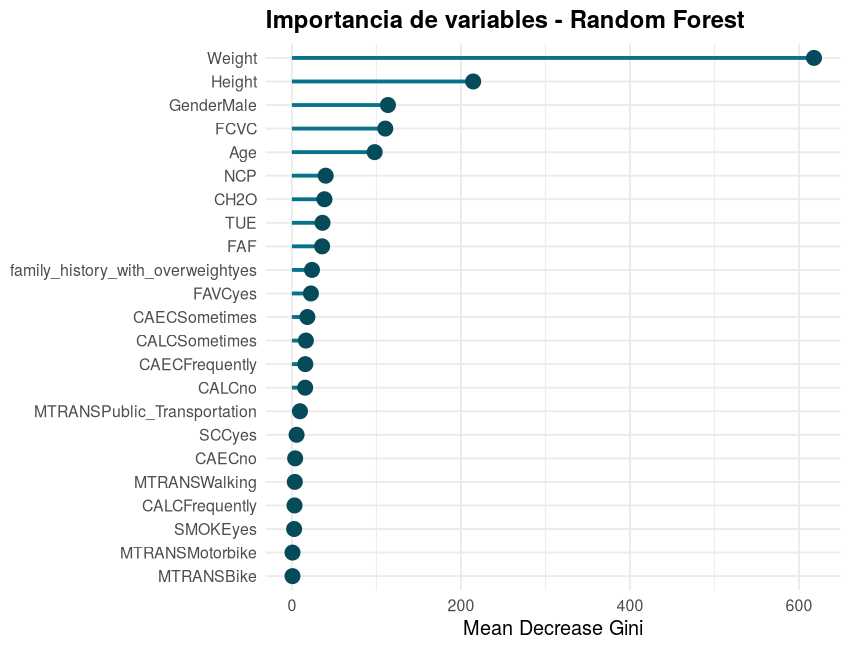
\includegraphics[width=\linewidth]{img/grafico-importancia-rf.png}\\
      {\scriptsize\color{cNavy} Importancia de variables (Random Forest)}
    \end{column}
  \end{columns}

  \vspace{0.2cm}
  \itemcheck{Peso y altura dominan}{CART y Random Forest coinciden: \texttt{Weight} y
    \texttt{Height} son los predictores más fuertes, lógico porque la clase se deriva del
    IMC (peso / altura\textsuperscript{2}).}
\end{frame}

% ============================================================
% 8. PREDICCIONES
% ============================================================
\activarnav{4}
\begin{frame}
  \seccionpill{\faIcon{magic}\ \ Predicciones con Random Forest}
  \vspace{0.15cm}

  \begin{columns}[T]
    \begin{column}{0.48\textwidth}
      \itemcheck{Muestra del set de prueba}{6 personas elegidas al azar:
        \textbf{6 de 6 aciertos}.}
      \vspace{2pt}
      \begin{center}
      \scriptsize
      \begin{tabular}{ll}
        \toprule
        \textbf{Real} & \textbf{Predicción} \\
        \midrule
        Obesity\_Type\_I      & Obesity\_Type\_I \\
        Obesity\_Type\_III    & Obesity\_Type\_III \\
        Insufficient\_Weight  & Insufficient\_Weight \\
        Overweight\_Level\_II & Overweight\_Level\_II \\
        Obesity\_Type\_I      & Obesity\_Type\_I \\
        Overweight\_Level\_II & Overweight\_Level\_II \\
        \bottomrule
      \end{tabular}
      \end{center}
    \end{column}
    \begin{column}{0.50\textwidth}
      \itemcheck{Persona nueva (hipotética)}{Varón de 27 años, 1.72\,m, 88\,kg,
        historial familiar de sobrepeso, poca actividad física.}
      \vspace{4pt}
      \begin{center}
      \tikz\node[fill=cNavy, rounded corners=6pt, text=white, inner sep=8pt,
                 text width=0.85\linewidth, align=center]
        {{\small Predicción:}\\[2pt]
         {\bfseries Overweight\_Level\_II}\\[2pt]
         {\small probabilidad \textbf{85.4\,\%}}};
      \end{center}
      {\scriptsize IMC $\approx$ 29.7, coherente con el rango de esa categoría.}
    \end{column}
  \end{columns}
\end{frame}

% ============================================================
% 9. CONCLUSIONES
% ============================================================
\activarnav{5}
\begin{frame}
  \seccionpill{\faIcon{lightbulb}\ \ Conclusiones}
  \vspace{0.15cm}

  \itemcheck{Random Forest es el mejor modelo}{96.9\,\% de accuracy y Kappa 0.964 en
    prueba; SVM lineal queda muy cerca (94.3\,\%).}
  \itemcheck{Los modelos simples se quedan cortos}{CART (78.3\,\%) no captura bien las
    fronteras entre niveles con un solo árbol; un ensamble o un margen lineal lo logran.}
  \itemcheck{LDA tiene una limitación real}{Avisó \textit{variables are collinear} por las
    dummies con niveles muy raros, aunque igual alcanzó 87.9\,\%.}
  \itemcheck{caret unifica todo el flujo}{Misma partición, validación cruzada y métricas
    para los cinco algoritmos: la comparación es justa y reproducible.}

  \vspace{0.1cm}
  \portadapill{\normalsize ¡Gracias!}
\end{frame}

\end{document}
